\chapter{SL: Regression}

\section{Polynomial Curve Fitting}

\begin{customArrayStretch}{1.5}
\begin{longtable}{l l l}

\hline\endfirsthead
\hline\endhead
\hline\endfoot
\hline
\caption*{Notations} \\
\endlastfoot

$N$ & number of observations (in training set) & known \\ \hline

$M$ & order of polynomial & hyper-param \\ \hline

$\bm{x} \equiv (x_1, \cdots , x_N)^\top$ & set of observations & known \\ \hline

$\bm{t} \equiv (t_1, \cdots , t_N)^\top$ & set of values for the observations & known \\ \hline

$\bm{w} \equiv (w_0, \cdots , w_M)^\top$ & weights (polynomial coefficients) & unknown (param) \\ \hline

$\hat{x}$ & new input data & \\ \hline

$\hat{t}$ & predicted value & \\ \hline

\end{longtable}
\end{customArrayStretch}

\begin{figure}[H]
    \centering
    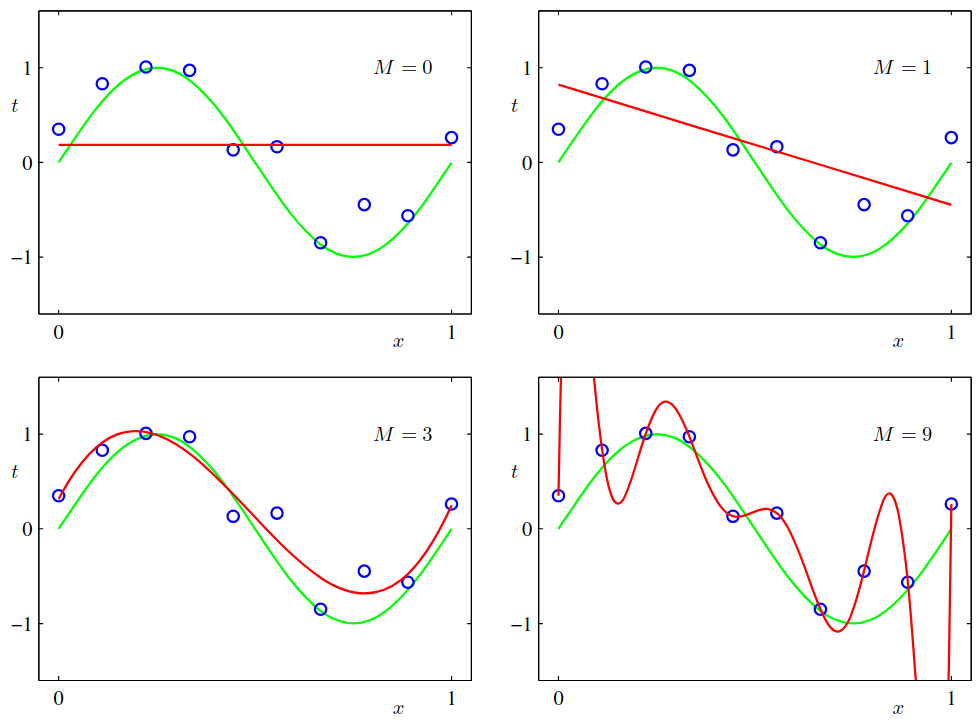
\includegraphics[
        width=\linewidth,
        height=10cm,
        keepaspectratio,
    ]{images/regression/poly-curve-m-vals.png}
    \caption*{
        Plots of polynomials having various orders $M$ fitted to the data set
        \cite{ml/book/Pattern-Recognition-And-Machine-Learning/Christopher-M-Bishop}
        \\
        \textcolor{green}{green curves}: original $\sin(2\pi x)$ curve 
        \hfill \vrule \hfill
        \textcolor{blue}{blue dots}: data points
        \hfill \vrule \hfill
        \textcolor{red}{red curves}: prediction polynomial 
    }
\end{figure}

\begin{enumerate}
    \item Polynomial function:
    $
        \hat{t}_i 
        = y(x_i, \bm{w}) 
        = w_0 + w_1x_i + w_2x_i^2 + \cdots + w_M x_i^M 
        = \dsum ^M _{j=0} w_j x_i^j
    $
    \hfill \cite{ml/book/Pattern-Recognition-And-Machine-Learning/Christopher-M-Bishop}

    \item Error: 
    $
        E(\bm{w}) 
        = \dfrac{1}{2} \dsum_{n=1}^N (\hat{t}_n - t_n)^2
    $
    \hfill
    $
        \hat{t}_n = y(x_n, \bm{w})
    $
    \hfill \cite{ml/book/Pattern-Recognition-And-Machine-Learning/Christopher-M-Bishop}
    \begin{enumerate}
        \item $\dfrac{1}{2}$ is used instead of $\dfrac{1}{N}$ for mathematical convenience (while differentiation)
    \end{enumerate}

    \item We can solve the curve fitting problem by choosing the value of $\bm{w}$ for which $E(\bm{w})$ is as small as possible. 
    Because the error function is a quadratic function of the coefficients $\bm{w}$, its derivatives with respect to the coefficients will be linear in the elements of $\bm{w}$, and so the minimization of the error function has a unique solution, denoted by $\bm{w}^\ast$, which can be found in \textbf{closed form}. 
    The resulting polynomial is given by the function $y(x, \bm{w}^\ast)$.
    \hfill \cite{ml/book/Pattern-Recognition-And-Machine-Learning/Christopher-M-Bishop}

    \item 
    \hfill \cite{ml/book/Pattern-Recognition-And-Machine-Learning/Christopher-M-Bishop}
\end{enumerate}















